\chapter{Practical Implementation}
    This Chapter delves into the practical implementation of the discussed RL algorithms, focusing on simulating the quadcopter in Gazebo in a realistic environment and employing Ardupilot SITL simulation to replicate the actual flight controller. The integration of ROS plays a crucial role in facilitating communication between the RL agent and the flight controller.
    \section{Software Specifications}
    \color{black}
    The software used in this implementation:\\
    \begin{itemize}        
        \item Solidworks 2022 \cite{solidworks}
        \item ArduCopter 4.4.4 \cite{arducopter}
        \item Blender 4.0 \cite{blender}
        \item Gazebo11 11.14.0 \cite{Gazebo}
        \item MAVLink \cite{mavlink}
        \item Ubuntu 20.04 (Focal) \cite{ubutnu}
        \item ROS1 noetic 1.16.0 \cite{ros}
    \end{itemize}
    %#############################################################
    \section{Setting Up Gazebo-ROS Environment}
        One of the most popular open-source autopilot software packages is Ardupilot, which is used widely for controlling UAVs on a variety of flights. When combined with Software-in-the-Loop (SITL) simulation environments, Ardupilot makes it easier to test and validate UAV algorithms and applications in a virtual environment before deploying them in the real world. This smooth integration facilitates innovation in autonomous flying operations, improves reliability, and speeds up development cycles. SITL simulations are used to verify the functionality of the RL algorithm to securely test new algorithms and identify technical defects.
        %##################################################
        \subsection{Creating 3D Model of the Drone's Environment}
        \color{black}
        A realistic 3D model of the drone's surroundings was generated in Gazebo11 to replicate flight in a real-world setting. Using the Polycam application, a 3D model of the lab where the drone flies was created by utilizing the LiDAR sensor built into the latest iPhone (Figure 4.1). This approach closely mimics actual flying conditions in the simulated environment, allowing for almost realistic simulation outcomes.
        \begin{figure}[H]
            \centering
            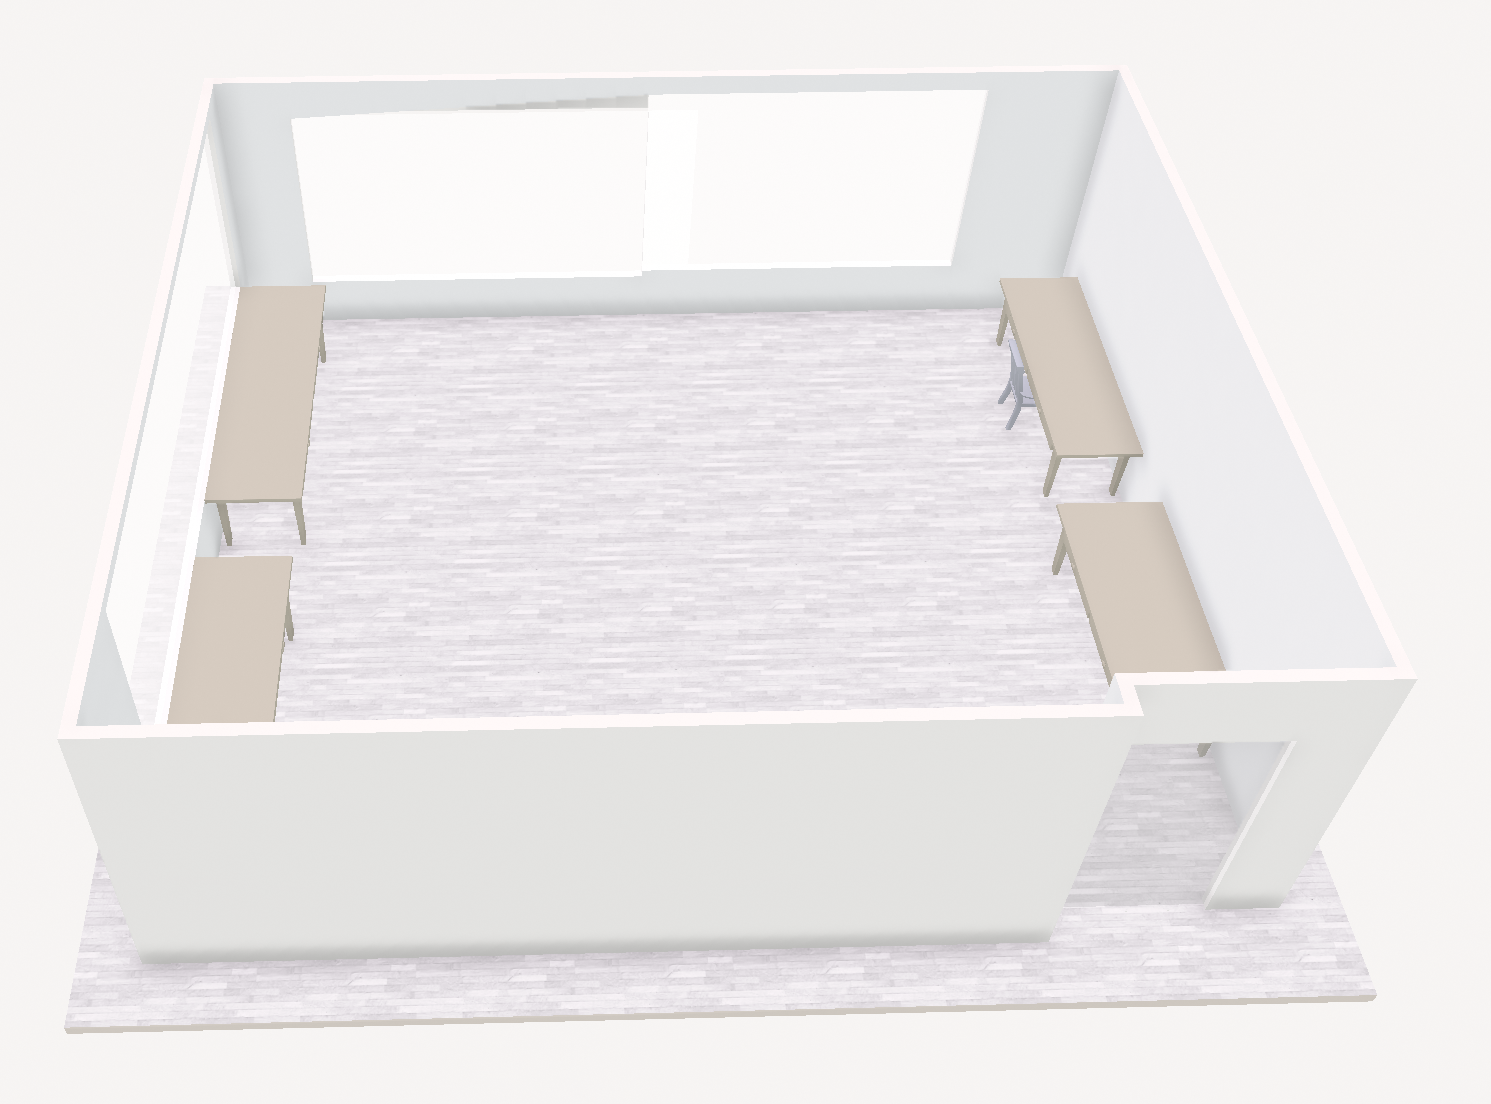
\includegraphics[width=0.6\linewidth]{Images/3D Model.png}
            \caption{Polycam 3D Model}
            \label{poly}
        \end{figure}
        The 3D model was then imported into Blender after being saved as a GLTF file. The modeled netted cage and the room's 3D model are integrated seamlessly in Blender (Figure 4.2). By following this procedure, an accurate simulation environment that accurately mimics the real-world surroundings and physical restrictions of the drone's operational environment is ensured.
    %##############################################################
        \subsection{Modelling Netted Cage in Solidworks}
        \color{black}
        The drone's flying area is a 6x6x3 meter netted cage with metal bars that have a 50x50 mm square cross-section. To accurately recreate the netted cage, the metal bars, and nets were precisely modeled as separate parts in SolidWorks before being put together into a single assembly. Through precise modeling, the physical structure is accurately recreated, allowing for accurate simulations and assessments of the drone's performance in the restricted area.
        \begin{figure}[H]
            \centering
            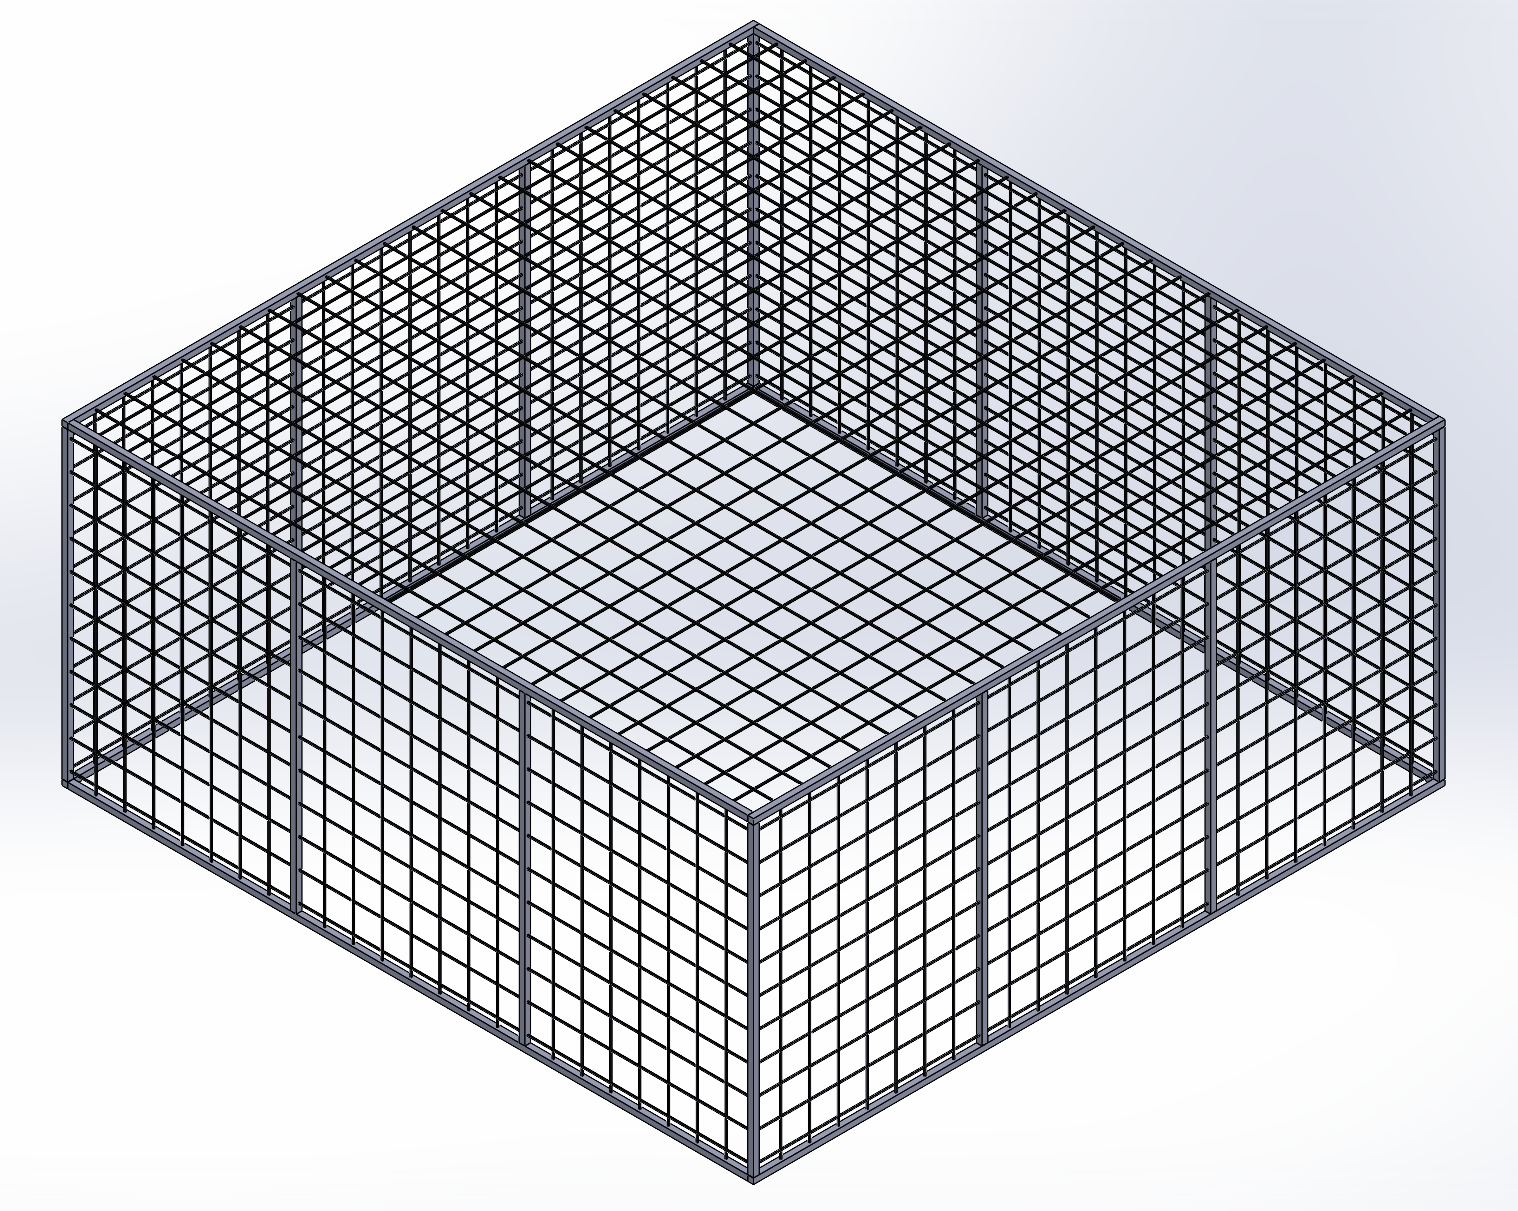
\includegraphics[width=0.6\linewidth]{Images/net.png}
            \caption{Netted Cage Assembly}
            \label{cage}
        \end{figure}
        To make integration with Blender's Polycam model easier, the assembly was then saved as an STL file. It requires SDF, Collada, and texture files to load the model into Gazebo11. These necessary files were produced by running the "SDF Exporter" Python script (see Appendix B.1) in Blender.
        \begin{figure}[H]
            \centering
            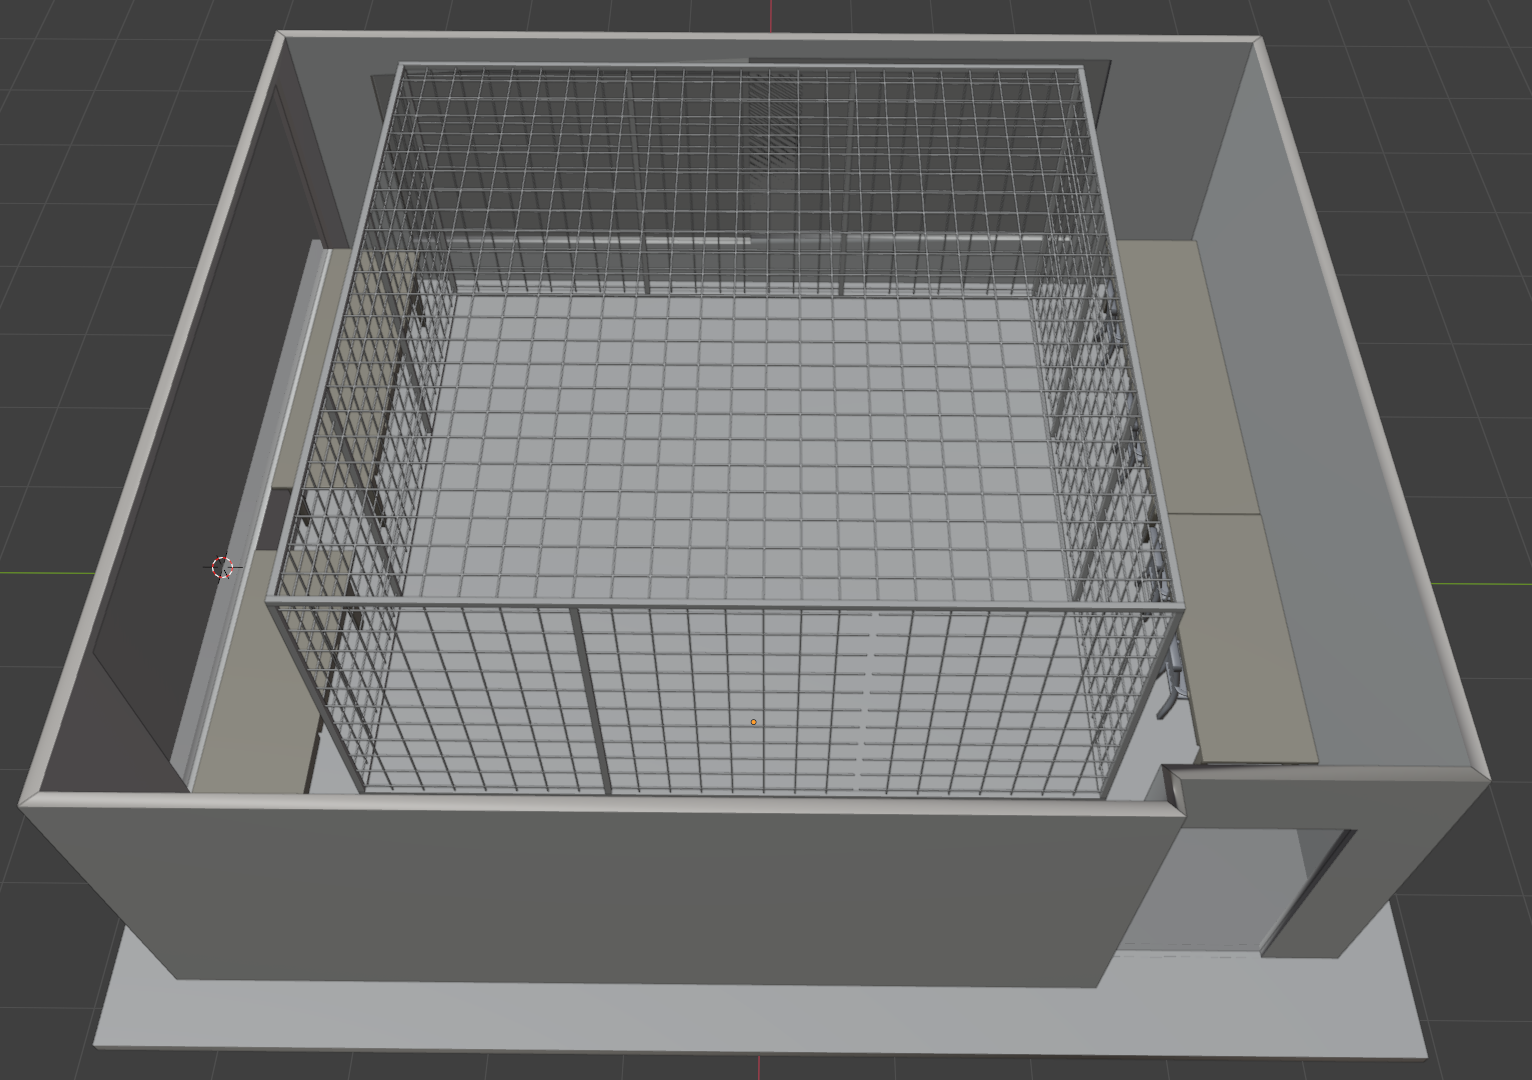
\includegraphics[width=0.6\linewidth]{Images/Blender.png}
            \caption{3D Model Inside Blender}
            \label{blender}
        \end{figure}
        The resulting files were then used to create a new Gazebo model, and a new environment containing the 3D model and the ArduPilot Iris Copter was produced. Realistic training and testing conditions within the Gazebo simulation environment are made possible by this process, which guarantees the smooth integration of the drone model and the simulated environment.
        \begin{figure}[H]
            \centering
            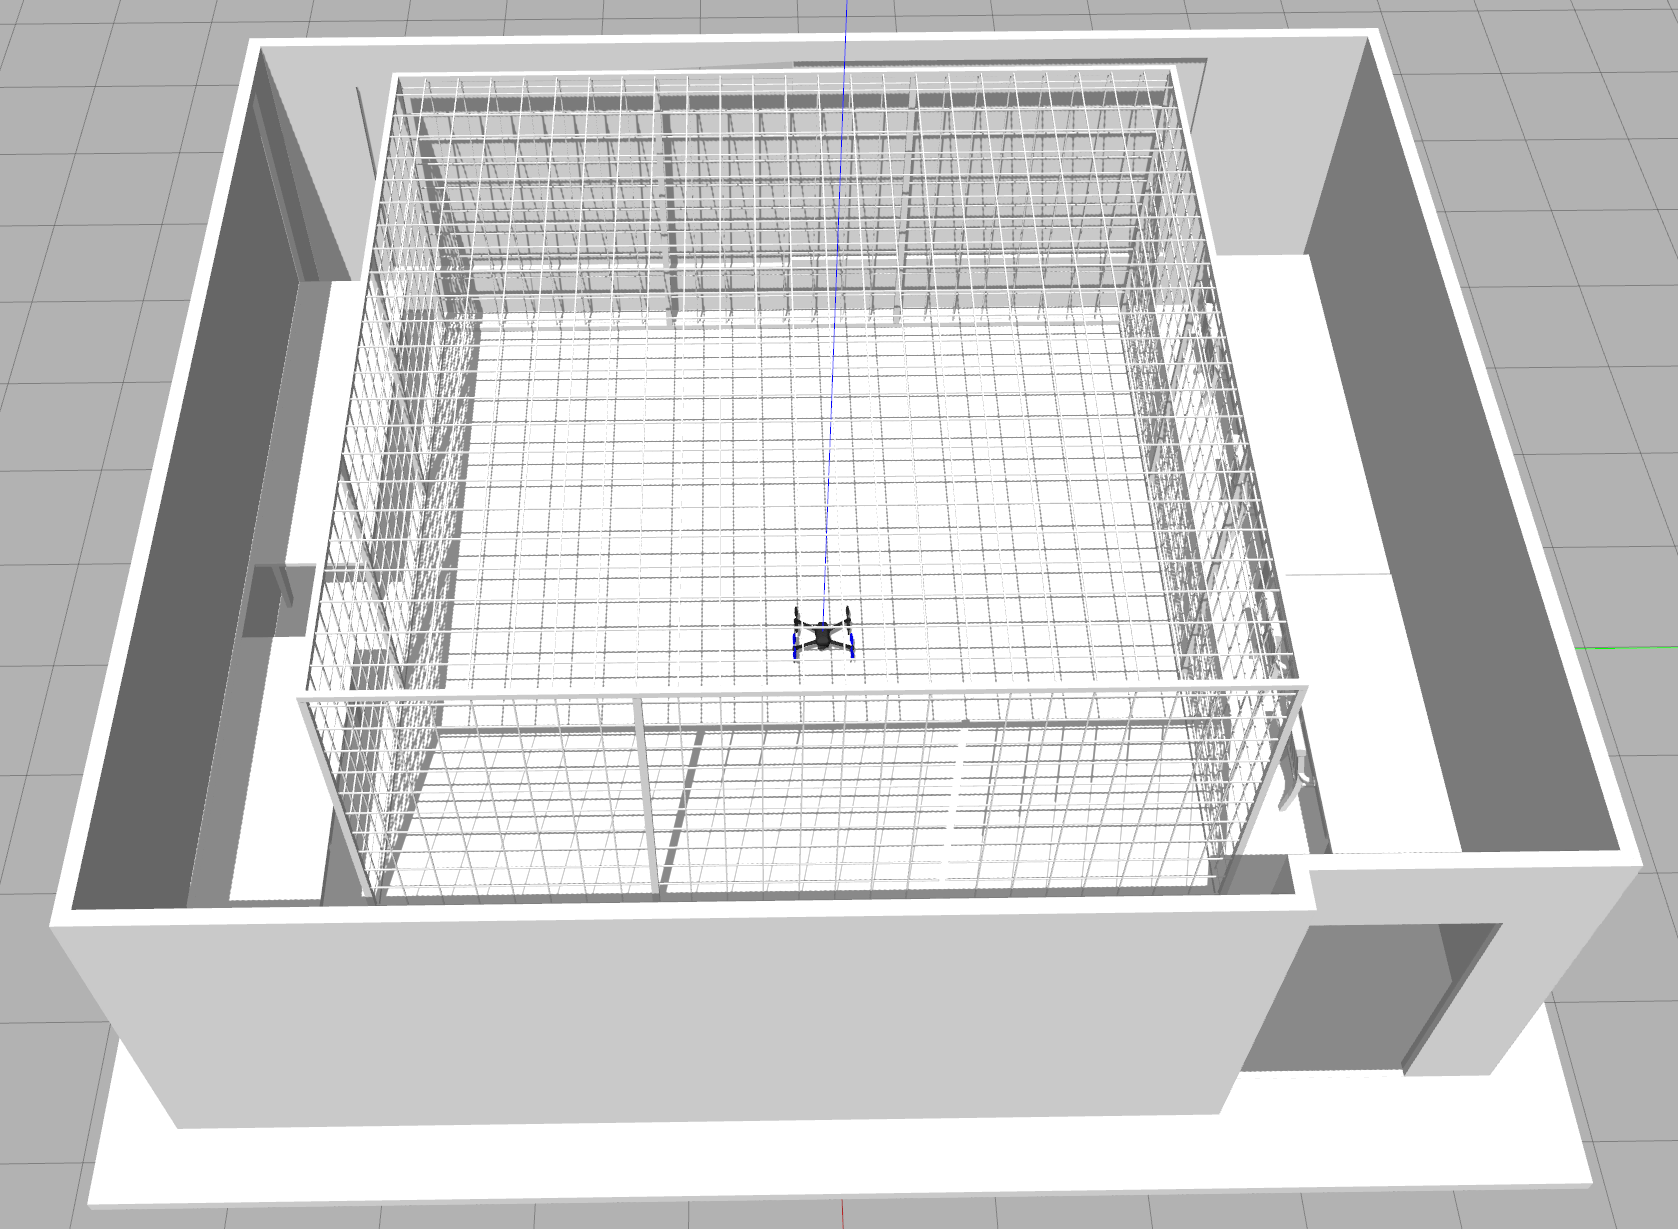
\includegraphics[width=0.6\linewidth]{Images/Gazebo.png}
            \caption{Gazebo Simulation Environment}
            \label{gazebo}
        \end{figure}
%############################################################
        \subsection{Testing the Environment}
        \color{black}
        Comprehensive testing was carried out utilizing Ardupilot SITL simulation to guarantee the environment's flawless operation before starting RL model testing. On a local setup, a SITL instance was initiated along with Gazebo, all of which were connected over the TCP protocol.

QGC acts as the ground station to monitor the drone's GPS position, change parameters, enable MAVLink protocol communication, and log flight information. On the other side, Gazebo serves as a physics simulator, simulating actual physics and displaying how the drone behaves in the virtual world.\\

Furthermore, the establishment of MAVROS communication created the necessary topics for commands to be sent to and received from the flight controller. To facilitate message communications among ROS publishers and subscribers, a C++ script was run to start a spiral flight pattern (see Appendix A.1).\\

In addition, a CSV file had echoes of the MAVROS topics that recorded position, speed, and attitude data. Then, using tools like Matlab, this data was plotted and compared with intended behaviors to analyze and visualize the drone's actual performance against expected behaviors (see Appendix C.1).
        \begin{figure}[H]
            \centering
            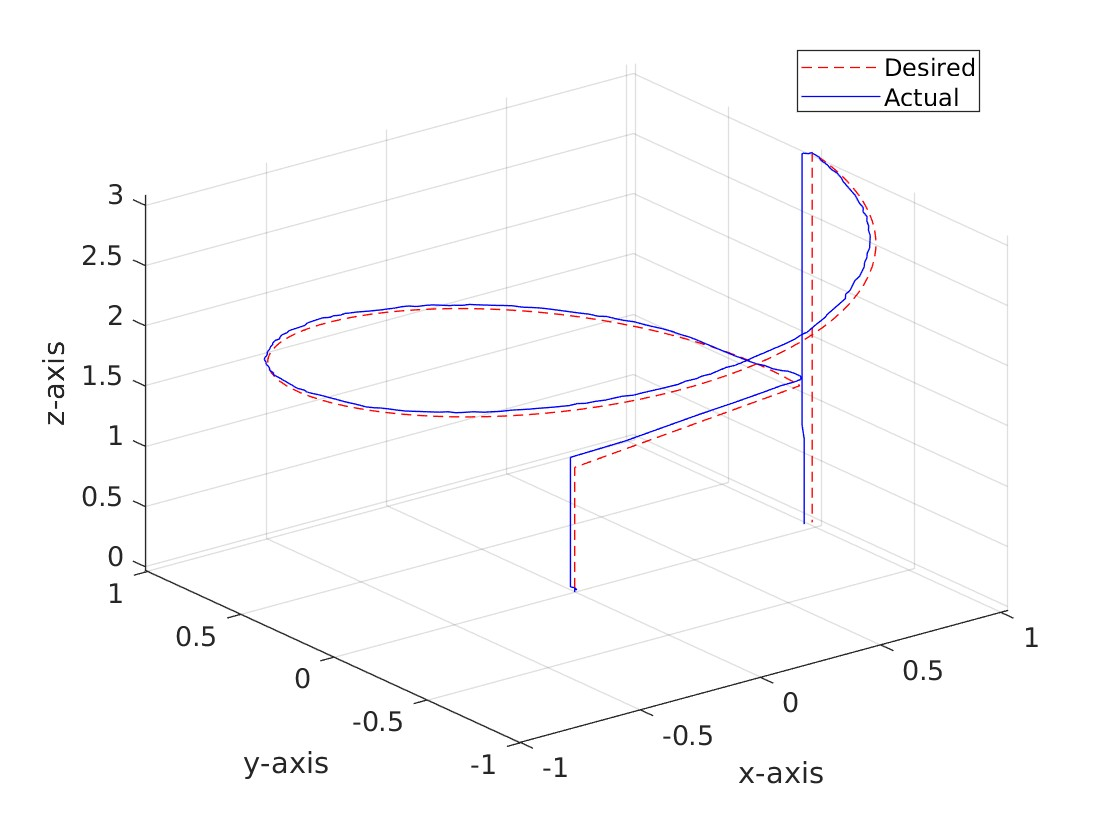
\includegraphics[width=0.6\linewidth]{Images/traj.jpg}
            \caption{Actual vs Desired Trajectory}
            \label{trajj}
        \end{figure}
        The position plot shows that the drone was able to track the desired trajectory with a small error in position
        \begin{figure}[H]
            \centering
            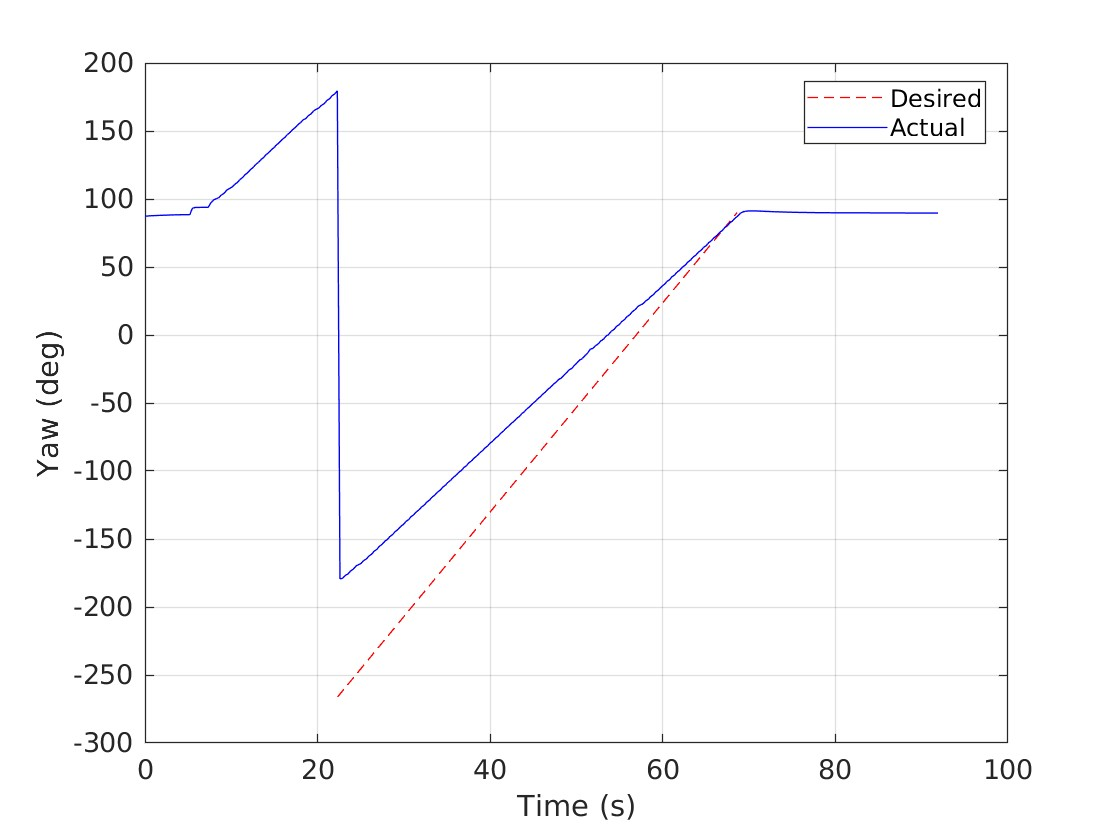
\includegraphics[width=0.6\linewidth]{Images/yaw.jpg}
            \caption{Actual vs Desired Yaw}
            \label{yaw}
        \end{figure}
        The yaw plot shows that the drone couldn't match the desired yaw angles however it reached the same desired end point. The test run was successful and the environment is ready to start testing the RL agents obtained.
    %#########################################################
\clearpage